\documentclass[10pt,twocolumn,letterpaper]{article}

\usepackage{cvpr}
\usepackage{times}
\usepackage{epsfig}
\usepackage{graphicx}
\usepackage{amsmath}
\usepackage{amssymb}

% Include other packages here, before hyperref.

% If you comment hyperref and then uncomment it, you should delete
% egpaper.aux before re-running latex.  (Or just hit 'q' on the first latex
% run, let it finish, and you should be clear).
\usepackage[breaklinks=true,bookmarks=false]{hyperref}

\cvprfinalcopy % *** Uncomment this line for the final submission

\def\cvprPaperID{****} % *** Enter the CVPR Paper ID here
\def\httilde{\mbox{\tt\raisebox{-.5ex}{\symbol{126}}}}

% Pages are numbered in submission mode, and unnumbered in camera-ready
%\ifcvprfinal\pagestyle{empty}\fi
\setcounter{page}{1}
\begin{document}

%%%%%%%%% TITLE
\title{Free-hand Sketch Recognition Classification}

\author{Wayne Lu\\
Stanford University \\
{\tt\small waynelu@stanford.edu}
% For a paper whose authors are all at the same institution,
% omit the following lines up until the closing ``}''.
% Additional authors and addresses can be added with ``\and'',
% just like the second author.
% To save space, use either the email address or home page, not both
\and
Elizabeth Tran\\
Stanford University\\
{\tt\small eliztran@stanford.edu}
}

\maketitle
%\thispagestyle{empty}

%%%%%%%%% ABSTRACT
\begin{abstract}

People use sketches to express and record their ideas. Free-hand sketches are usually drawn by non-artists using touch sensitive devices rather than purpose-made equipments; thus, making them often highly abstract and exhibit large intraclass deformations. This makes automatic recognition of sketches more challenging than other areas of image classification because sketches of the same object can vary based on artistic style and drawing ability. In addition, sketches are less detailed and thus harder to distinguish than photographs. Using a publicly available dataset of 20,000 sketches across 250 classes from Eitz et al. ~\cite{eitz2012hdhso}, we are applying convolutional neural networks (CNNs) in order to improve performance to increase the recognition accuracy on sketches drawn by different people. In our experiments, we analyze the effects of several hyperparmeters on overall performance using a residual network (ResNet) approach.  
 
\end{abstract}

%%%%%%%%% BODY TEXT
\section{Introduction}
Sketching is one of the primary methods people use to communicate visual information. Since the era of primitive cave paintings, humans have used simple illustrations to represent real-world objects and concepts. Sketches are often abstract and stylized, varying based on artistic ability and style. In addition, sketches emphasize defining characteristics of real-world objects and ignore features which are either less important or more difficult to draw. For example, texture is almost never rendered unless it is important for recognition, such as the spikes on a hedgehog. In this way, sketches can be interpreted as a distillation of human visual recognition schemas.

Sketch recognition attempts to recognize the intent of the user while allowing the user to draw in an unconstrained manner. This allows for the user to not have to spend time being trained how to draw on the system, nor will the system need to be trained on how to recognize each users particular drawing style. Deciphering freehand sketches can be viewed under the lens of image category recognition, a well studied problem in the computer vision community.  

However, the sketch recognition problem differs from traditional photographic image classification. First, sketches are less visually complex than photographs. Whereas color photographs have three color channels per pixel, sketches are encoded as either black-and-white or grayscale. Photographs contain visual information throughout the image whereas sketches consist primarily of blank space. Second, sketches and photographs have different sources of intraclass variation. Whereas photographic image classification faces obstacles such as camera angle, occlusion, and illumination, photographs are still grounded in reality. On the other hand, sketches differ based on artistic style, which is unique to every artist. While people can agree on what an object looks like, how they ultimately render the object can vary significantly.

In this paper, we explore the use of deep convolutional neural networks (DCNN) architectures for sketch recognition. Since DCNNs are primiarly designed for photos, we demonstrate that DCNNs can be used for sketches, but there needs to be some modifications. Here, we are going to modify the ResNet architecture in order for it used for sketches. To the best of our knowledge, ResNets have not been utilized for online sketch recognition.


%-------------------------------------------------------------------------
\section{Related Work}

Since SketchPad ~\cite{sutherland1964sketchpad}, sketch recognition has introduced sketching as a means of human computer interaction. Computer vision has since tried different approaches to achieve better results in multiple application areas. Eitz et al. ~\cite{eitz2012hdhso} was able to demonstrate classification rates can be achieved for computational sketch recognition by using local feature vectors, bag of features sketch representation and SVMs to classify sketches. Schneider et al.~\cite{schneider2014sketch} then modified the benchmark proposed by Eitz et al ~\cite{eitz2012hdhso}  by making it more focused on how the image should like, rather than the original drawing intention, and they also used SIFT, GMM based on Fisher vector encoding, and SVMs to achieve sketch recognition.

Previous work on sketch recognition generally extracts hand crafted features from the sketch followed by feeding them to a classifier.  Convolutional neural networks (CNN) have emerged as a powerful framework for feature representation and recognition ~\cite{krizhevsky2012imagenet}.  Convolutional neural networks are a type of neurobiologically inspired feed-forward artificial neural network which consist of multiple layers of neurons,  and  the neurons in each layer are then collected into sets. At the input layer, where the data gets introduce to the CNN, these neuron sets map to small regions of input image. Deeper layers of the network can be composed of local or global pooling (fully-connected) layers which combine outputs of the neuron sets from previous layer. The pooling is typically achieved through convolution-like operations. Deep neural networks (DNN), especially CNNs, can automatically learn features instead of manually extracting features and its multi layers learning can get more effective expression. When it comes to CNN design, the trend in the past few years has pointed in one direction: deeper networks ~\cite{krizhevsky2012imagenet}. This move towards deeper networks  has been beneficial for many applications. The most prominent application has been object classification, where the deeper the neural network, the better the performance. However, current existing CNNs are designed for photos, and they are trained on a large amount of data to avoid overfitting. 

Traditional CNNs are limited in depth, as empirical results showed that training error increased with depth, suggesting that deeper networks become increasingly hard to train. This problem was addressed by He et al. with the introduction a deep residual network architecture, which uses shortcut connections to allow convolutional layers to approximate residuals rather than actual mappings \cite{hekaming2016}. Their model was able to set new records for both the ImageNet and COCO datasets, and through the application of residual networks, CNNs with over a thousand layers have been trained.

Sketches, on the other hand, require special model architectures. In 2012, Eitz et al.~\cite{eitz2012hdhso} released the largest sketch object dataset. Since its release, a number of approaches have been proposed to recognize freehand sketches.  In Yu et al. ~\cite{yu2016sketch}, they proposed Sketch-a-Net, a different type of CNN that is customizable towards sketches. While Sarvadevabhatla et al. ~\cite{sarvadevabhatla2015freehand} used two popular CNN architectures (ImageNet and a modified LeNet) to fine-tuned their parameters on the TU-Berlin sketch dataset in order to extract deep features from CNNs to recognize hand-drawn sketches. 


 The current state-of-the-art is ~\cite{seddati2016deepsketch}, where propose a ConvNet for classification but they also include in feature extraction and similarity search. 


%-------------------------------------------------------------------------

\section{Method}
\subsection{Residual networks}
Deep residual networks were used by He et al. to great success on image classification challenges, including ImageNet and CIFAR-10 \cite{hekaming2016}. Residual networks differ from standard neural networks in that instead of learning a target mapping $x \rightarrow H(x)$, they attempt to learn the residual mapping $F(x) = H(x) - x$. The original mapping is then recovered as $H(x) = F(x) + x$. These residual mappings are implemented as modular residual units which consist of a stack of convolutional layers and a shortcut connection which carries the original input $x$. When the convolutional layers produce output of the same dimensions, $x$ is simply passed through with an identity projection. When the output dimensions change, such as in the case of pooling or increased stride, $x$ is projected to the new dimensions via a 1x1 convolution followed by average pooling.

 \begin{figure}[h]
	\begin{center}
	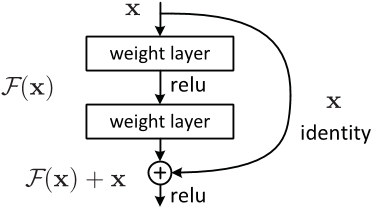
\includegraphics[width=.5\linewidth]{resnet}
	\caption{Model of a 2-layer basic residual unit using the identity projection \cite{hekaming2016}. }
	\end{center}
\end{figure}

\subsection{Wide residual networks}
Wide residual networks were proposed by Zagoruyko and Komodakis as an alternative to deep residual networks \cite{zagoruyko2016wide}. The authors widen a network by increasing the number of filters per convolutional layer while decreasing the overall depth in the network, in contrast to the original ResNet architecture which was thin and deep. Properly tuned wide networks have fewer parameters than deep networks, thus requiring less memory to store and less time to train. In this project, we briefly experiment with the effects of trading depth for width with a wide variant of our base architecture.

\subsection{Dropout}
Dropout was introduced by Srivastava et al. as a simple stochastic regularization method \cite{srivastava2014dropout}. Dropout reduces the number of active neurons during training time by setting the output of a neuron to 0 with probability $p$. Intuitively, this forces the next layer in the network to train on sparser and more randomized input, which helps prevent overfitting on the training data. In the original formulation of dropout, zeroing does not occur during inference. Instead, outputs are simply scaled by $(1 - p)$ to their expected values. This requires additional computation during inference time, which is undesirable. As a solution, inverted dropout combines zeroing and scaling output by $1 / (1 - p)$ during training so that no additional computation is required during inference. Our model makes use of periodic inverted dropout for regularization.

\subsection{Batch normalization}
Batch normalization is a method of centering and normalizing inputs to each convolutional layer, which helps make the network more resilient to learning rate choices and poor network weight initialization \cite{ioffe2015batch}. The batch normalization algorithm is parameterized by scaling factor $\gamma$ and mean shift $\beta$, both of which are trainable. During training time, the algorithm uses mini-batch mean and variance to normalize the batch. It then scales the normalized inputs by $\gamma$ and $\beta$. During inference, a running average of mean and variance from the training data is used for normalization instead. By mitigating the effects of internal covariate shift, in which the distribution of the layer inputs changes deeper in the network, the network is able to train faster with less need to finely tune hyperparameters.

\subsection{Softmax cross-entropy loss}
Softmax cross-entropy loss is one of the standard loss function for classification problems. For a single example, given the class score output $s_1, s_2, \dots, s_C$ of a neural network, the scores are converted to probabilities $p_1, \dots, p_C$ via the softmax function 
\begin{align}
p_i = \sigma(s_i) = \frac{e^{s_i}}{\sum_{j = 1}^C s_j}
\end{align}
 Let $y$ be the correct class. Then, the cross-entropy loss is 
 \begin{align}
 L = -\log p_y = -\log \left( \frac{e^{s_y}}{\sum_{j = 1}^C s_j} \right)
 \end{align}
  Cross-entropy loss has the advantage of being differentiable, in contrast with SVM loss which is not. In addition, cross-entropy loss aims to drive all incorrect class scores to 0 while SVM loss is only concerned with increasing the correct class score above a certain margin.

\subsection{Adam optimization}
Adam is an adaptive learning rate optimization algorithm which incorporates both moving average of moments to achieve per-parameter scaling of updates \cite{kingma2014adam}. In particular, it increases the step size of variables with slow moving updates and decreases the step size of fast moving updates. It is similar to the RMSProp optimization, but also incorporates momentum updates. Given learning rate $\alpha$, decay parameters $\beta_1, \beta_2$, and numerical stability constant $\varepsilon$, the update step is
\begin{align}
m &:= \beta_1 m + (1 - \beta_1) \nabla x \\
v &:= \beta_2 v + (1 - \beta_2) (\nabla x)^2 \\
x &:= x - \alpha \frac{m}{\sqrt{v} + \varepsilon}
\end{align}

The full version of the optimization algorithm also introduces bias terms to help the algorithm initialize its states at the beginning of training.

\subsection{Convolutional network architectures}
In this project, we explore four different convolutional network architectures. The basic architecture consists of an initial 7x7 convolutional layer. This layer is then followed by a series of 12 3x3 residual units, for a total of 25 convolutional layers (not including layers used for residual projection). Every third residual unit, the feature map size is halved by increasing stride while the number of filters is doubled. At the end of the network, global average pooling is used and followed by a fully connected layer to output logits for softmax cross-entropy loss. Dropout is applied on the initial input, every third residual unit, and before the fully connected layer.

The wide variant of the architecture replaces the 12 residual units with 8 residual units of doubled width, for a total of 17 convolutional layers. Dimension changes occur every second residual unit rather than every third unit, and dropout is applied every second unit rather than every third. The rest of the architecture remains the same.

The widest variant of the architecture consists of an initial 7x7 convolutional layer followed by 3 wide 3x3 residual units. The residual units are followed by a bottleneck layer then a 2048-filter layer, for a total of 9 convolutional layers. As in the basic architecture, global average pooling and a fully connected layer are used to generate logits. Dropout is applied on the initial input, after each residual unit, and before the fully connected layer.

The fourth fusion variant is almost identical to the basic architecture, but doubles the width of the last set of 3 residual units to 1024, as a more controlled experiment on the effects of width.

In all four architectures, convolutional layers are followed by batch normalization.

\begin{figure}[h]
\begin{center}
\begin{tabular}{l | r}
Layer & Output Size \\ \hline \hline
Input	& 128x128x1\\
Dropout &  \\
7x7 conv, 64, /2	 & 64x64x64\\
3x3 residual unit, 64	& 64x64x64\\
3x3 residual unit, 64 & \\
3x3 residual unit, 64	& \\
Dropout	&  \\
3x3 residual unit, 128, /2 & 32x32x128\\
3x3 residual unit, 128 & \\
3x3 residual unit, 128 &\\
Dropout & \\
3x3 residual unit, 256, /2 & 16x16x256\\
3x3 residual unit, 256 & \\
3x3 residual unit 256	 & \\
Dropout	& \\
3x3 residual unit, 512, /2	& 8x8x512\\
3x3 residual unit, 512	&\\
3x3 residual unit, 512& \\
8x8 Average Pooling	& 512\\
Dropout& 	\\
Fully connected, 250	& 250
\end{tabular}
\caption{Basic convolutional network architecture.}
\end{center}
\end{figure}

\begin{figure}[h]
\begin{center}
\begin{tabular}{l | r}
Layer & Output Size \\ \hline \hline
Input	& 128x128x1\\
Dropout &  \\
7x7 conv, 128, /2	 & 64x64x128\\
3x3 residual unit, 128	& 64x64x128\\
3x3 residual unit, 128 & \\
Dropout	&  \\
3x3 residual unit, 256, /2 & 32x32x256\\
3x3 residual unit, 256 & \\
Dropout & \\
3x3 residual unit, 512, /2 & 16x16x512\\
3x3 residual unit, 512 & \\
Dropout	& \\
3x3 residual unit, 1024, /2	& 8x8x1024\\
3x3 residual unit, 1024	&\\
8x8 Average Pooling	& 1024\\
Dropout& 	\\
Fully connected, 250 	& 250
\end{tabular}
\caption{Wide convolutional network architecture.}
\end{center}
\end{figure}

\begin{figure}[h]
\begin{center}
\begin{tabular}{l | r}
Layer & Output Size \\ \hline \hline
Input	& 128x128x1\\
Dropout & \\
7x7 conv, 256, /2	 & 64x64x256\\
3x3 residual unit, 256	& 64x64x256\\
Dropout	&  \\
3x3 residual unit, 256, /2 & 32x32x256\\
Dropout & \\
3x3 residual unit, 512, /2 & 16x16x512\\
Dropout	& \\
1x1 conv, 256 & 16x16x256 \\
3x3 conv, 2048, /2 & 8x8x2048 \\
8x8 Average Pooling	& 2048\\
Dropout& 	\\
Fully connected, 250	& 250
\end{tabular}
\caption{Widest convolutional network architecture.}
\end{center}
\end{figure}

%-------------------------------------------------------------------------
\section{Dataset}
\begin{figure}[h]
	\begin{center}
	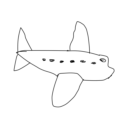
\includegraphics[width=0.5\linewidth]{airplane}
	\caption{Example sketch from the TU Berlin dataset.}
	\end{center}
\end{figure}

For this project, we are using a dataset of sketches collected by Eitz et al. \cite{eitz2012hdhso}. The dataset consists of 20,000 images evenly distributed across 250 different classes and was collected from 1,350 participants via Amazon Mechanical Turk, a crowdsourcing platform. Images are provided as 1111x1111px PNG files.

To make the dataset more manageable, we first resized every image to 128x128px using bilinear interpolation. For each class, there are 80 images which we divide in 48 training examples, 16 validation examples, and 16 test examples. To augment the low number of training examples, we generate additional examples by horizontally flipping the provided images, for a total of 96 training examples per class. This is similar to the data augmentation used by Seddati et al., who implemented training time image distortion through mirror and rotation \cite{seddati2015deepsketch}. In total, we used 24,000 training examples, 4,000 validation examples, and 4,000 testing examples, evenly distributed across the 250 classes. The images are read into memory and stored as grayscale 128x128x1 arrays. On loading, we also invert the images so that the behavior of our input dropout creates white space when zeroing inputs.

Even though the database covers a range of object categories, its major shortcoming comes from ambiguous drawn sketches ~\cite{schneider2014sketch} and overlapping object classes. For examples, the object classes include both "sea gull" and "flying bird." In order to address this problem, Rosalia et al. ~\cite{schneider2014sketch} were able to find a subset of 160 unambiguous object categories to make a more reliable benchmark. However, we are choosing to use all 250 object categories in order to compare our accuracies with other models. 
 
\begin{figure}[h]
	\begin{center}
	\includegraphics[width=.5\linewidth]{invert_colors_2}
	\caption{Example sketch of inverted with inverted color value that was fed into our model.}
	\end{center}
\end{figure}
 

%-------------------------------------------------------------------------

\section{Experiments}
\subsection{Dropout rates}
Our first set of experiments were focused on investing the effects of dropout rates on classification accuracy. In these experiments, we use the basic architecture with dropout rates of 0\%, 20\%, and 50\%. Each network is trained for 15 epochs with a training rate of 0.001 and for 5 epochs with a decayed training rate of 0.0001. After every epoch, validation accuracy is computed and the weights of the network are saved. After the training epochs, the set of weights with the highest validation accuracy are used to compute the test accuracy.

\begin{table}[h]
	\begin{center}
	\begin{tabular}{l | c}
	Dropout rate & Test accuracy \\ \hline \hline
	0\% & 0.651 \\
	20\% & 0.656 \\
	50\% & 0.653 \\
	\end{tabular}
	\caption{Test accuracies of varying dropout rates on the basic architecture.}
	\end{center}
\end{table}

The results show that varying dropout rate does not appear to have a noticeable effect on accuracy, as all test accuracies are within 1\% of each other. Instead, the effects of dropout manifest in the training accuracy curves, in which stronger dropout leads to slow convergence of training accuracy. This suggests that our model would benefit from increased model capacity to improve its representational power rather than from stronger regularization.

\begin{figure}[h]
	\begin{center}
	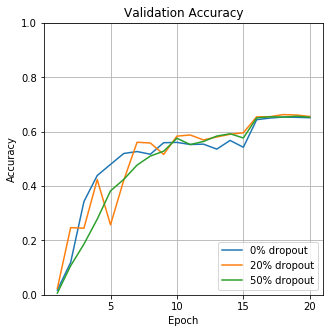
\includegraphics[width=0.75\linewidth]{dropout-val-acc}
	\caption{Validation accuracy curves for varying dropout rates. Note that the curves are nearly identical.}
	\end{center}
\end{figure}

\begin{figure}[h]
	\begin{center}
	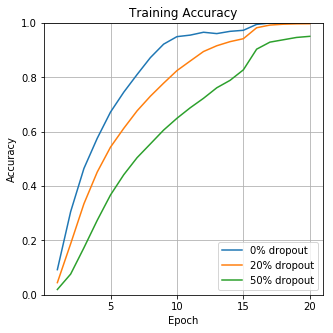
\includegraphics[width=0.75\linewidth]{dropout-train-acc}
	\caption{Training accuracy curves for varying dropout rates. Note that stronger dropout leads to slower learning rates.}
	\end{center}
\end{figure}

\subsection{Network depth}
The second set of experiments investigate the effects of network depth on classification accuracy. In this set of experiments, we use the four previously discussed architectures, each trained with 50\% dropout. Each network is trained for 15 epochs with a training rate of 0.001 or until loss plateaus, then trained for 5 epochs with a training rate of 0.0001 or until loss plateaus, which occurs first. As before, the weights are saved after every training epoch, and the set of weights with the highest validation accuracy are used to compute the test accuracy.

\begin{table}[h]
	\begin{center} 
	\begin{tabular}{l | c | c | c}
	Model & Depth & Parameters & Test accuracy \\ \hline \hline
	Basic & 25 & 17.6M & 0.653 \\
	Wide & 17 & 45.7M & 0.621 \\
	Widest & 9 & 11.5M & 0.588 \\
	Fusion & 25 & 20.2M & 0.653
	\end{tabular}
	\caption{Test accuracies of network architectures with varying depths.}
	\end{center}
\end{table}

The results show a clear correlation between network depth and classification accuracy. Increasing the width of the "wide" and "widest" networks was not enough to compensate for decreasing the depth. Notably, the wide network performed worse than the basic network, despite having almost 3 times as many parameters. These numbers do not necessarily contradict the results of Zuoruyko and Komodakis, as their work primarily focused on reducing the depth of networks with over 1000 layers. It could instead be said that our networks are still at a scale which would see more benefit from adding layers to introduce more non-linearity than from increasing width to increase the overall model capacity.

\subsection{Results comparison and analysis}
Of the experiments, our best performing model used the basic architecture with a 20\% dropout rate. It achieved a test accuracy of 65.6\%. In comparison, this is better than the original classifier proposed by Eitz et al. which utilized an SVM classifier trained on extracted SIFT features \cite{yesilbek2015svm}. However, state-of-the-art achieves much higher accuracy, with Seddati et al. reaching 75.4\% and 77.7\% cross-validation accuracy with their convolutional DeepSketch and DeepSketch 2 models \cite{seddati2015deepsketch} \cite{seddati2016deepsketch}. In addition, Yesilbek et al. were able to reach 71.30\% cross-validation accuracy using an SVM classifier trained on traditional image features \cite{yesilbek2015svm}.

\begin{table}[h]
        \begin{center}
        \begin{tabular}{l | c}
        Model & Accuracy \\
        \hline\hline
        SIFT+ SVM  ~\cite{eitz2012hdhso}  &  0.560 \\
        \textbf{Basic, 20\% dropout}& \textbf{0.656} \\
        IDM + SVM ~\cite{yesilbek2015svm} & 0.713 \\
        Human ~\cite{eitz2012hdhso} & 0.730 \\
        Multi-scale Multi-angle Voting ~\cite{Sadouk2016} &0.7543\\
        DeepSketch ~\cite{seddati2015deepsketch}  & 0.754\\
        DeepSketch2 ~\cite{seddati2016deepsketch} & 0.777\\
        \end{tabular}
        \end{center}
        \caption{Test accuracy comparison of our model versus other methods.}
\end{table}

Due to the large number of classes, we have omitted a confusion matrix. Instead, we computed the three most easily and least easily classified labels. 

\begin{table}[h]
        \begin{center}
        \begin{tabular}{l | c}
        Label & Accuracy \\
        \hline\hline
        Rollerblades & 1.0 \\
        Nose & 1.0 \\
        Zebra & 0.9375 \\ \hline
        Dragon & 0.1875 \\
        Seagull & 0.125 \\
        Panda & 0.0625
        \end{tabular}
        \end{center}
        \caption{Classification accuracies of the three most easily and three least easily classified labels}
\end{table}

Unsurprisingly, "seagull" is the second-worst label. Further examination reveals that its examples are misclassified 5 times as a pigeon, 3 times as a standing bird, twice as a flying bird, and once each as a syringe, duck, and canoe. This demonstrates the problems which arise from interclass overlap because for many people, there is no difference between drawing these varieties of birds. 

\begin{figure}[h]
	\begin{center}
	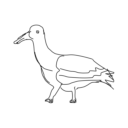
\includegraphics[width=0.3\linewidth]{seagull}
	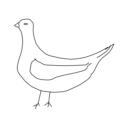
\includegraphics[width=0.3\linewidth]{pigeon}
	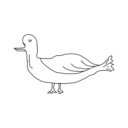
\includegraphics[width=0.3\linewidth]{standingbird}
	\caption{From left to right: a seagull, a pigeon, and a standing bird.}
	\end{center}
\end{figure}

"Panda," as the worst label, is an example of both intraclass variation and interclass overlap. Panda examples were misclassified as teddy bears 6 times, or one-third of the testing examples. In addition, the sketches span a large variety of poses, colorations, and artistic talent. In contrast, sketches of rollerblades all encompass the same general idea of a foot shaped object on top of circles, representing the boot and wheels of a rollerblade.

\begin{figure}[h]
	\begin{center}
	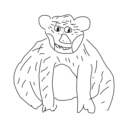
\includegraphics[width=0.3\linewidth]{panda1}
	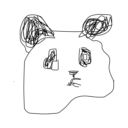
\includegraphics[width=0.3\linewidth]{panda2}
	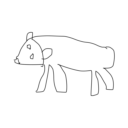
\includegraphics[width=0.3\linewidth]{panda3}
	\caption{Three images from the panda classification. Note the large variation in posing and coloring.}
	\end{center}
\end{figure}

%-------------------------------------------------------------------------
\section{Conclusion}

In this paper, we have presented our CNN architecture for freehand sketch recognition. From our results, we see evidence of the intraclass variation and interclass overlap caused by differences in artistic interpretation and scarcity of visual information which make sketch recognition challenging. In contrast, traditional image recognition faces the problems of variation and overlap caused by an overabundance of visual noise in photographs.

Our experiments show that deeper networks provide higher classification accuracy, with moderate dropout helping to reduce overfitting. Shallow wide networks, even with more parameters, perform worse. Unfortunately, due to the limits of time, we were unable to investigate networks deeper than 25 layers. However, both our results and other literature suggest that increasing depth will continue to yield better classification accuracy. In addition, more time was spent exploring different architectures than on fully tuning each architecture. Better hyperparameter tuning, as well as introduction of other forms of regularization such as L2 would likely also yield better classification accuracy.

The TU-Berlin dataset, though is the largest, is still relatively limited. However, some things that we can try next is use other networks to train on the TU- Berlin dataset, such as using VGG to train on sketches or the original architecture of ResNet. Our source code can be accessed at: https://www.github.com/krinkels/sketch-recognition


{\small
\bibliographystyle{ieee}
\bibliography{milestone}
}


\end{document}
